\chapter{Bayes' Theorem}

Let's say that you are holding two bags of marbles.
You know that one bag contains 60 white marbles and 40 red marbles. And you
know that the other holds 10 white marbles and 90 red marbles. You
don't know which is which -- and you can't see the marbles.
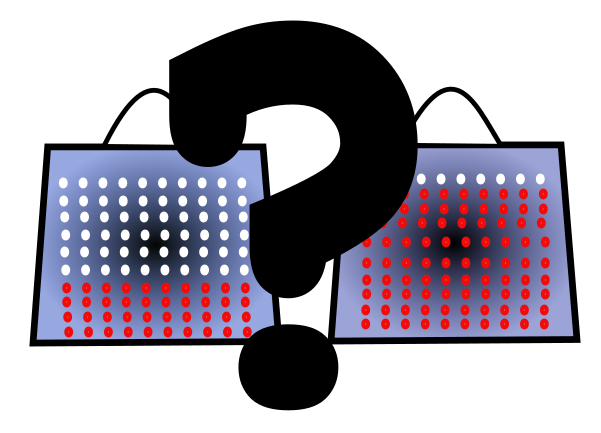
\includegraphics[width=0.8\textwidth]{M_Bags.png}

I say ``Guess which bag is mostly red marbles.'' You pick one.

``What is the probability that this is the bag that is mostly red marbles?''
 You think "50 percent and there is
also a 50 percent probabilitiy that it is the mostly-white-marbles bag.''

Then you pick one marble from the bag. It is red. Now you must
update your beliefs. It is more likely that this is the
mostly-red-marbles bag. What is the probability now?

Bayes Theorem gives you the rule for updating your beliefs based on
new data.

\section{Bayes Theorem}

Let's say you have two events or conditions $C$ and $D$. $C$ is
``The person has a cough'' and $D$ is ``The person is waiting to see a doctor.''

Using the chain rule of probability, we now have two ways to calculate $p(C \text{ AND } D)$:
% ADD: add rule of probability to index

$$p(C \text{ AND } D) = p(C | D) p(D)$$

(The probability the person is at the doctor multiplied by the probability they have a cough if they are at the doctor.)

or 

$$p(C \text{ AND } D) = p(C | D) p(D)$$

(The probabilitiy the person has a cough multiplied by the probabilitiy they are at the doctor if they have a cough.)
% ADD: This needs a little more explanation
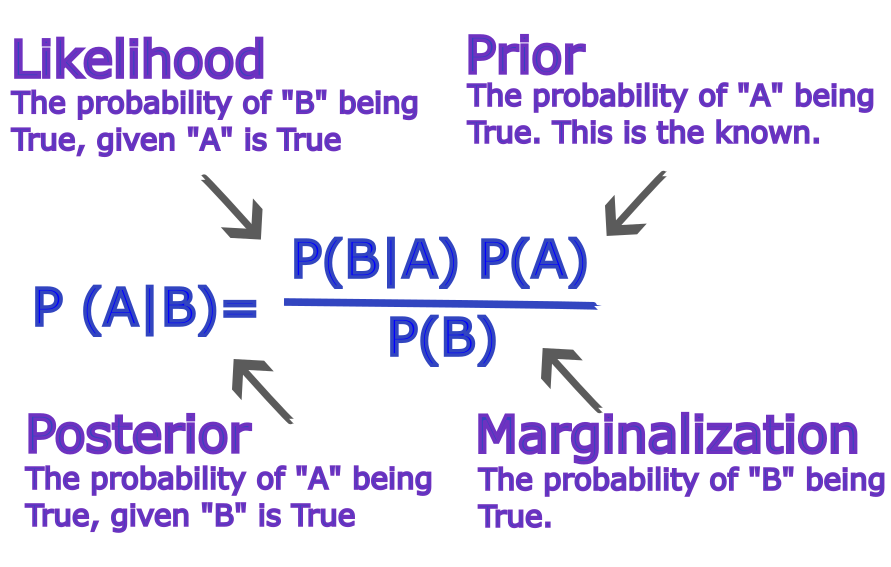
\includegraphics[width=0.8\textwidth]{Probability.png}

Thus:

$$p(D | C) = \frac {p(C | D)p(D)}{P(C)}$$

Now you can calculate $p(D | C)$ (in this case, the probability that
you are waiting to see a doctor given that you have a cough.) if you
know:

\begin{itemize}
\item $p(C | D)$ (The probability that you have a cough given that you are waiting to see a doctor)
\item $p(D)$ (The probability that you are waiting for a doctor for any reason.)
\item $p(C)$ (The probability that you have a cough anywhere)
\end{itemize}

Pretty much all modern statistical methods (including most artificial
intelligence) are based on this formula, which is known as Bayes'
Theorem. It was written down by Thomas Bayes before he died in
1761. It was then found and published after his death.

\includegraphics[width=0.8\textwidth]{Bayes.png}

\section{Using Bayes' Theorem}

Back to the example at the beginning. To review:

\begin{itemize}
\item There are two bags that look exactly the same.
\item Bag W has 60 white marbles and 40 red marbles.
\item Bag R has 10 white marbles and 90 red marbles.
\item You pull one marble from the selected bag -- it is red.
\end{itemize}

What is the probability that the selected bag is Bag R? Intuitively,
you know that the probability is now more than 0.5. What is the exact
number?

In terms of conditional probability, we say we are looking for ``the probability
that the selected bag is Bag R, given that you drew a red marble?'' or
$p(B_R | D_R)$, where $B_R$ is ``The selected bag is Bag R'' and $D_R$ is
``You drew a red marble from the selected bag''.

From Bayes' Theorem, we can write:

$$p(B_R | D_R) = \frac{ P(D_R | B_R) P(B_R) } {P(D_R)}$$

$P(D_R | B_R)$ is just the probability of drawing a red marble given that the
selected bag is Bag R. That is easy to calculate: There are 100
marbles in the bag, and 90 are red. Thus $P(D_R | B_R) = 0.9$.

$P(B_R)$ is just the probability that you chose Bag R before you drew
out a marble. Both bags look the same, so $P(B_R)= 0.5$. This is
called \textit{the prior} because it represents what you thought the
probability was before you got more information.

$P(D_R)$ is the probability of drawing a red marble. There was 0.5
probability that you put your hand into Bag W (in which 40 of the 100
marbles are red) and a 0.5 probability that you put your hand into Bag
R (in which 90 of the 100 marbles are red).  So

$$P(D_R) = 0.5 \frac{40}{100} + 0.5 \frac{90}{100} = 0.65$$

Putting it together:

$$p(B_R | D_R) = \frac{ P(D_R | B_R) P(B_R) } {P(D_R)} = \frac{(0.9)(0.5)}{0.65} = \frac{9}{13} \approx 0.69$$

Thus, given that you have pulled a red marble, there is about a 69\% chance
that you have selected the bag with 90 red marbles.

\section{Confidence}

Bayes' Theorem, then, is about updating your beliefs based on
evidence.  Before you drew out the red marble, you selected one bag
thinking it might contain 90 red marbles. How certain were you? 0.0 being complete disbelief and 1.0 entirely
confidence, you were 0.5. After pulling out the red marble, you were about 0.69
confident that you had chosen the bag with 90 red marbles.

The question ``How confident are you in your guess?'' is very
important in some situations. For example in medicine, diagnoses often
lead to risky interventions. Few diagnoses come with 100\% confidence.
All doctors should know how to use Bayes' Theorem. 
% ADD: This is why doctors are taught to think hourses not zebras

And in a trial, a jury is asked to determine if the accused person is
guilty of a crime. Few jurors are ever 100\% certain. In some trials, Bayes'
Theorem is a really important tool.

